
\chapter{Week1}

\section{Monday}\index{Monday_lecture}

\subsection{Introduction to Stochastic Process}
\paragraph{Course Information}
\begin{itemize}
\item
Instructor: Prof. Masakiyo Miyazawa
\item
Course Venue: Chengdao 208
\item
Office Hour: 3-5pm, Monday, at Daoyuan 514
\end{itemize}
\paragraph{Motivation of Stochastic Process}
\begin{itemize}
\item
capture randomness;
\item
characterize randomness influences in real systems;
\item
improve the design and operation of such systems.
\end{itemize}

\begin{example}[Coin Tossing Example]
Consider a scenario where someone bets money by coin tossing.
Assume that
\begin{itemize}
\item
Head and tail occur likely and independently;
\item
Get or loss money by head or tail, respectively;
\item
There is no limit for money to bet.
\end{itemize}
The goal of this people is to double the money he initialy obtains.
Therefore, the best policy is that he should stop the betting 
when the money becomes double of the initial.
The question is that is this policy \emph{realizable}?
\begin{itemize}
\item
By probability theory, we could argue that such event will eventually happen with probability one.
\item
However, this policy is actually not realizable.
This is because the expected time for the realization of this event is infinite!
See the Figure.~\ref{fig:1:1} for three simulation cases of betting.
\end{itemize}
\begin{figure}[H]
\centering
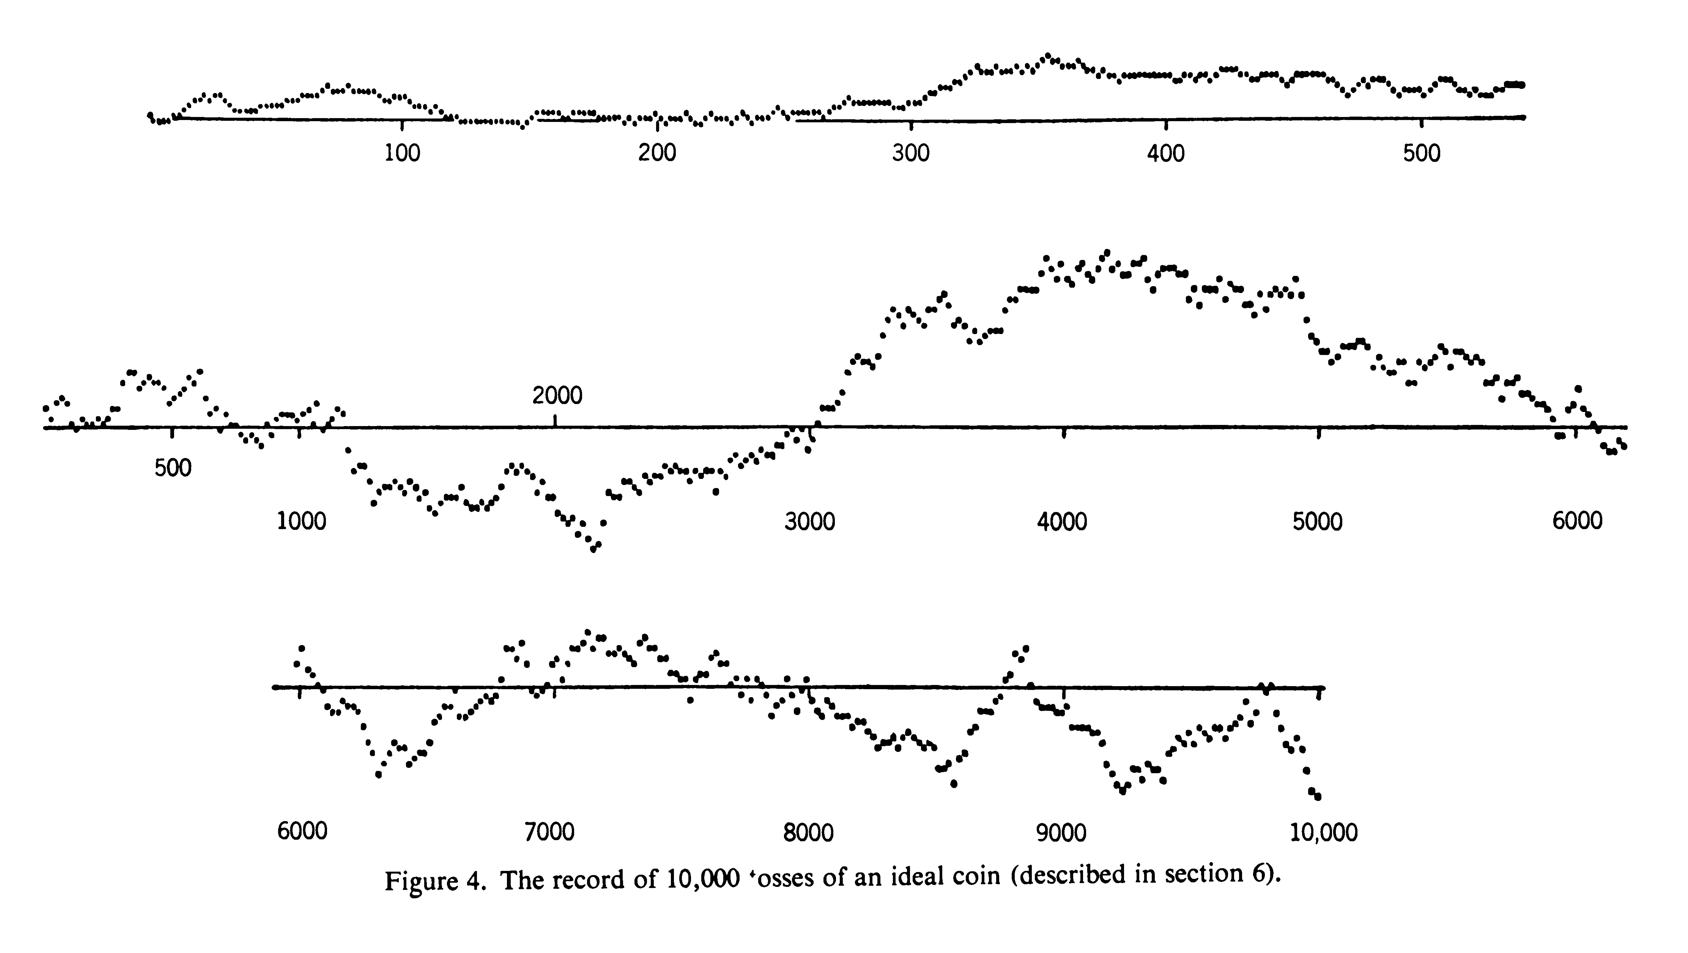
\includegraphics[width=0.8\textwidth]{week1/p_1}
\caption{Simulation of coin tossing for 10000 times}
\label{fig:1:1}
\end{figure}
\end{example}
\paragraph{Course Outline}
Mathematical Model for random phenomena: probability space.
\begin{itemize}
\item

\end{itemize}
Two ways to constructor a probability space $(\Omega,\mathcal{F},\mathbb{P})$:
\begin{itemize}
\item
Measure theory based: $\mathcal{F}=\mathcal{B}(\Omega)$.

Standard for stochastic processes. (indexed by time)
\item
Functional Analysis based: 
Define the probability $\mathbb{P}$ by functional mapping:
\[
\begin{array}{ll}
\phi:&\mathcal{C}_b(\Omega)\to\mathbb{R}_+\\
\text{with}&f\in\mathcal{C}_b(\Omega): \Omega\to S~\mbox{(state space)}
\end{array}
\]
Also we could define the norm for $f$ and $\phi$:
\[
\begin{array}{ll}
\|f\|=\sup\limits_{x\in\Omega}~f(x),
&
\|\phi\|=\sup\limits_{\|f\|\le 1}\|f\|
\end{array}
\]
Suitable for Gaussian Processes (indexed by vector).
\end{itemize}

Discrete time stochastic processes~(DTSP):
\begin{itemize}
\item
random walk and limit theorems
\item
Conditional expectation, martingale, stopping time
\item
DTMC and applications;
\end{itemize}

Continuous time stochastic processes~(CTSP):
\begin{itemize}
\item
Possion process, Brownian motion, martingale
\item
Stochastic analysis; predictability, semi-martingale, stochastic integral, Ito's formula
\item
CTMC and applications.
\end{itemize}

W. Rudin Real and Complex Analysis.

\subsection{Mathematical Background}
\paragraph{Logics}
Get familar with the operations $\land,\lor,\lnot,\equiv,\Rightarrow$:
\begin{itemize}
\item
$P\Rightarrow Q$ is T iff $\lnot P\lor Q$ is T;
\item
$\lnot(P\Rightarrow Q)\equiv P\land (\lnot Q)$;
\item
$\lnot (\forall x\in A, P(x)) \equiv \exists x\in A, \lnot P(x)$
\end{itemize}

\paragraph{Limits}
Get familar with $\sup,\inf,\lim\sup,\lim\inf,\lim$:
\begin{itemize}
\item
$\sup\limits_{n\ge 1}a_n=\bar{a}$ iff
\[
\left\{
\begin{aligned}
\forall\varepsilon>0,\exists n_0, \forall n\ge n_0, a_n<\bar{a}+\varepsilon\\
\forall\varepsilon>0,\forall n\ge1, \exists n_1\ge n, \bar{a}-\varepsilon<a_{n_1}\\
\end{aligned}
\right.
\]
and $\inf\limits_{n\ge 1}a_n=-\sup\limits_{n\ge 1}(-a_n)$.
\item
$\limsup\limits_{n\to\infty} a_n$ and $\liminf\limits_{n\to\infty} a_n$.
\item
$\lim\limits_{n\to\infty}a_n=a$ iff $\limsup\limits_{n\to\infty} a_n=a=\liminf\limits_{n\to\infty} a_n$.
Or equivalently,
\[
\forall\varepsilon>0,\exists n_0\ge1, \forall n\ge n_0,
\qquad
|a_n-a|<\varepsilon.
\]
\end{itemize}
\paragraph{Set Theory}
Given mapping $f:A\to B$
\begin{itemize}
\item
Onto mapping: $f(A)=B$;
\item
One-to-one mapping: $f(x)=f(y)$ implies $x=y$
\item
Berstein's theorem:
if there are both one-to-one mappings from $A$ to $B$ 
and from $B$ to $A$, then $\|A\|=\|B\|$.
\end{itemize}

\subsection{Random Phenomena}
The key feature for random phenomena is \emph{multiple outcomes}.
Define possible outcomes as follows.
\begin{definition}[Sample Space]
An outcome is called a sample.
The set of all possible samples is called a \emph{sample space}, denoted by $\Omega$.
\end{definition}


\begin{example}
Toss a coin for $n$ times.
Define $H$ for head and $T$ for tail.
The possible outcome can be denoted as
$
\omega=(\omega_i)_{i=1}^n,$
with 
$
\omega_i\in\{H,T\}
$.
The sample space $\Omega$ is the set of all these $\omega$, with $2^n$ elements.
\end{example}

In order to characterize behaviours such as coin tossing, we need to define how to choose a sample from $\Omega$. 
The statistical way is to assign a number to each sample which represents the corrresponding likelihood to choose it, called a \emph{probability}. 
The formal definition of probability relies on the distribution function:
\begin{definition}[Distribution]\label{def:1:2}
Assume $\Omega$ to be finite or countably infinite set.
Define a function $p:\Omega\to[0,1]$ as follows:
\begin{itemize}
\item
$p(\omega)\ge0,\forall \omega\in\Omega$
\item
$\sum_{\omega\in\Omega}p(\omega)=1$
\end{itemize}
then $p(\cdot)$ is called a \emph{distribution} over $\Omega$.
Moreover, $(\Omega,p(\cdot))$ is called a \emph{discrete probability space}, and $p(\omega)$ denotes the probability that the event $\omega$ occurs.
\end{definition}
%\begin{definition}[Discrete Probability Space]
%$(\Omega, p(\cdot))$ is a mathematical model for a random phenomenon, called a discrete probability space.
%\end{definition}
\begin{remark}
This definition cannot be directly applied into the uncountable sample space $\Omega$. For instance, consider the unlimited coin tossing behaviour.
The uncountable $\Omega$ defined as follows:
\[
\Omega=\{0,1\}^{\infty}\supseteq[0,1].
\]
Since any event $\omega$ happens with the same probability as the coin is fair, 
one can argue that $p(\omega)=0,\forall\omega\in\Omega$, which contradicts to the second condition in Definition~\ref{def:1:2}.
\end{remark}

\paragraph{Ideas to define a probability for uncountable sample space}
Use limiting operation when faced uncountable.



\begin{definition}[$\sigma$-field]
A set $\mathcal{F}$ containing subsets of $\Omega$ is called a $\sigma$-field if:
\begin{enumerate}
\item
$\Omega\in\mathcal{F}$;
\item
$\mathcal{F}$ is closed under complement, i.e., 
$A\in\mathcal{F}$ implies $\Omega\setminus A\in\mathcal{F}$;
\item
$\mathcal{F}$ is closed under infinite union operation, i.e.,
$A_i\in\mathcal{F},i\ge1$ implies $\cup_{i=1}^\infty A_i\in\mathcal{F}$.
\end{enumerate}
\end{definition}

\begin{definition}[Probability Measure]
A function $\mathbb{P}:\mathcal{F}\to\mathbb{R}$ is called a \emph{probability measure} on $(\Omega,\mathcal{F})$ if
\begin{itemize}
\item
$\mathbb{P}(\Omega)=1$;
\item
$\mathbb{P}(A)\ge0,\forall A\in\mathcal{F}$;
\item
$\mathbb{P}$ is $\sigma$-additive, i.e., when $A_i\in\mathcal{F},i\ge1$ and $A_i\cap A_j=\emptyset,\forall i\ne j$, 
\[
\mathbb{P}\bigg(
\bigcup_{i=1}^\infty A_i
\bigg)
=
\sum_{i=1}^\infty\mathbb{P}(A_i).
\]
\end{itemize}
where $\mathbb{P}(A)$ is called the \emph{probability of the event} $A$.
\end{definition}

\begin{definition}[Probability Space]
A \emph{probability space} is a triple $(\Omega,\mathcal{F},\mathbb{P})$, where
\begin{itemize}
\item
$\Omega$ is a set of samples, called the sample space;
\item
$\mathcal{F}$ is a $\sigma$-field, a collection of events;
\item
$\mathbb{P}$ is a probability measure, which assigns probability to events.
\end{itemize}
\end{definition}
\begin{remark}
Here we give an explicit construction of the \emph{canonical} probability space, as 
the $\sigma$-field induced by $\Omega$ may not be unique.
\begin{itemize}
\item
When $\Omega$ is discrete, we can construct \emph{the} probability space $(\Omega,\mathcal{F},\mathbb{P})$ such that
\[
\mathcal{F}=2^{\Omega},
\quad
\mathbb{P}(A)=\sum_{\omega\in A}p(\omega),~~A\in\mathcal{F}.
\]
\item
Otherwise, we define $\mathcal{F}$ with no ``redundancy''.
When $\Omega$ is a \emph{topological space}, with $\mathcal{O}$ being the \emph{topology} of $\Omega$, define
\[
\mathcal{B}(\Omega)=\sigma(\mathcal{O})\equiv
\text{the minimal $\sigma$-field on $\Omega$ containing $\mathcal{O}$}.
\]
Let $\mathcal{F}=\mathcal{B}(\Omega)$ and construct the associated probability measure $\mathbb{P}$.
Then $(\Omega,\mathcal{F},\mathbb{P})$ is the \emph{canonical} probability space.
\end{itemize}
\end{remark}
Next we give some reviewings on the topological space:
\begin{definition}
A \emph{topological space} $(X,\mathcal{T})$ consists of a (non-empty) set $X$, and a family of subsets of $X$ (``open sets'' $\mathcal{T}$) such that
\begin{enumerate}
\item
$\emptyset,X\in\mathcal{T}$
\item
$U,V\in\mathcal{T}$ implies $U\bigcap V\in \mathcal{T}$
\item
If $U_\alpha\in\mathcal{T}$ for all $\alpha\in\mathcal{A}$, then $\bigcup_{\alpha\in\mathcal{A}}U_\alpha\in\mathcal{T}$.
\end{enumerate}
When $A\in\mathcal{T}$, $A$ is called the open subset of $X$. The $\mathcal{T}$ is called a \emph{topology} on $X$.
\end{definition}

\begin{example}
Let $(X,d)$ be any metric space, and define
\[
\mathcal{T}=\{
O\subseteq X:~
\forall x\in O, \exists\varepsilon>0,
\mathbb{B}_{\varepsilon}(x)\subseteq O
\}
\]
It's clear that $(X,\mathcal{T})$ is a topological space.
\end{example}




\begin{definition}[Topological Space]
A is open when
\[
\forall x\in A,\exists B\in\mathcal{O}, x\in B\subseteq A
\]
\end{definition}


Define the distribution function for $\Omega=\mathbb{R}$:

Define the probability of an event $A\in\mathcal{B}(\mathbb{R})$.


\subsection{Random variable and test functions}
\[
\mathbb{E}~f(X),\qquad f\in\mathcal{C},
\]
where $f$ is called a \emph{test function} of $X$.









